\section{Newton's Method}\label{S:3.8.Newtons}

\begin{goals}% NEED GOALS
\item If we are unable to solve an equation algebraically, how can we approximate the solutions of the equation using calculus?
\end{goals}

%--------------------------------------
% SUBSECTION INTRODUCTION
%--------------------------------------
\subsection*{Introduction}

Solving equations is one of the most important things we do in mathematics, yet we are surprisingly limited in what we can solve analytically.  For instance, equations as simple as $x^5+x+1=0$ or $\cos(x) =x $ cannot be solved by algebraic methods in terms of familiar functions.  Fortunately, there are methods that can give us \textit{approximate} solutions to equations like these.  These methods can usually give an approximation correct to as many decimal places as we like. In Section~\ref{S:1.3.Continuity} we learned about the Bisection Method.  This section focuses on another technique (which generally works faster), called Newton's Method.

\begin{pa} \label{PA:3.8}
The graph of $f(x)$ is shown in Figure \ref{fig:3.8.PA1}. 
\ba
	\item Draw the tangent line to $f(x)$ at $x=a_0$ and extend the tangent line until it intersects the $x$ axis. 
	\item Label the $x$-intecept of the tangent line as $a_1$. What do you notice about $a_1$ and the root of $f(x)$?
	\item Now draw the tangent line to $f(x)$ at $x=a_1$ and extend the tangent line until it intersects the $x$ axis.
	\item  Label the $x$-intecept of the tangent line as $a_2$. What do you notice about $a_2$ and the root of $f(x)$?
	\item If we continue this process, what do think happens to the distance between $a_n$ and the root of $f(x)$?
\ea
\end{pa} 
\afterpa

\begin{marginfigure}[-6cm]
\margingraphics{figures/3_8_PA1.pdf}
\caption{The graph of $y=f(x)$ in Preview Activity \ref{PA:3.8}}\label{fig:3.8.PA1}
\end{marginfigure} % PREVIEW ACTIVITY

%-------------------------------------------
% SUBSECTION NEWTON'S METHOD
%-------------------------------------------
\subsection*{Newton's Method}

Newton's Method is built around tangent lines.  The main idea is that if $x$ is sufficiently close to a root of $f(x)$, then the  tangent line to the graph at $(x,f(x))$ will cross the $x$-axis at a point closer to the root than $x$.  

We start Newton's Method with an initial guess about roughly where the root is.  Call this $x_0$. (See Figure~\ref{fig:newt1}-(a).)  Draw the tangent line to the graph at $(x_0,f(x_0))$ and see where it meets the $x$-axis. Call this value $x_1$.  Then repeat the process -- draw the tangent line to the graph at $(x_1, f(x_1))$ and see where it meets the $x$-axis. (See Figure \ref{fig:newt1}-(b).) Call this value $x_2$.  Repeat the process again to get $x_3$, $x_4$, etc.  This sequence of points will often converge rather quickly to a root of $f$.  

\begin{marginfigure}[0cm] % MARGIN FIGURE
\begin{center}
\subfloat[]{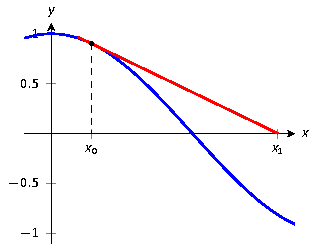
\includegraphics[scale=.8]{figures/fignewt1a}}

\subfloat[]{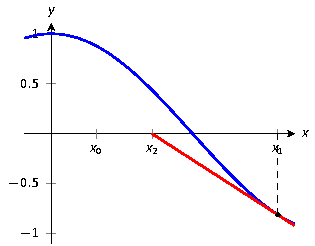
\includegraphics[scale=.8]{figures/fignewt1b}}

\subfloat[]{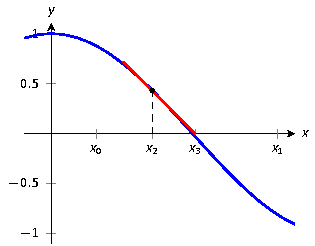
\includegraphics[scale=.8]{figures/fignewt1c}}
\caption{Demonstrating the geometric concept behind Newton's Method.}\label{fig:newt1}
\end{center}
\end{marginfigure}

We can use this \textit{geometric} process to create an \textit{algebraic} process.  Let's look at how we found $x_1$.  We started with the tangent line to the graph at $(x_0,f(x_0))$.  The slope of this tangent line is $\fp(x_0)$ and the equation of the line is
$$y=\fp(x_0)(x-x_0)+f(x_0).$$
This line crosses the $x$-axis when $y=0$, and the $x$--value where it crosses is what we called $x_1$. So let $y=0$ and replace $x$ with $x_1$, giving the equation: 
$$ 0 = \fp(x_0)(x_1-x_0)+f(x_0).$$ 
Now solve for $x_1$:
$$x_1=x_0-\frac{f(x_0)}{\fp(x_0)}.$$
Since we repeat the same geometric process to find $x_2$ from $x_1$, we have
$$x_2=x_1-\frac{f(x_1)}{\fp(x_1)}.$$
In general, given an approximation $x_n$, we can find the next approximation, $x_{n+1}$ as follows:
$$x_{n+1} = x_{n} - \frac{f(x_{n})}{\fp(x_{n})}.$$

We summarize this process as follows.

\concept{Newton's Method} % CONCEPT
{Let $f$ be a differentiable function on an interval $I$ with a root in $I$. To approximate the value of the root, accurate to $d$ decimal places:\index{Newton's Method}
\begin{enumerate}
\item Choose a value $x_0$ as an initial approximation of the root. (This is often done by looking at a graph of $f$.)
\item	 Create successive approximations iteratively; given an approximation $x_n$, compute the next approximation $x_{n+1}$ as $$x_{n+1} = x_n - \frac{f(x_n)}{\fp(x_n)}.$$
\item Stop the iterations when successive approximations do not differ in the first $d$ places after the decimal point.
\end{enumerate}
} % end concept

\marginnote{Newton's Method is not infallible. The sequence of approximate values may not converge, or it may converge so slowly that one is ``tricked'' into thinking a certain approximation is better than it actually is. These issues will be discussed at the end of the section.}

Let's practice Newton's Method with a concrete example.

\begin{example} \label{Ex:3.8.Eg1}
Approximate the real root of $x^3-x^2-1=0$,  accurate to the first $3$ places after the decimal, using Newton's Method and an initial approximation of $x_0=1$.

\solution To begin, we compute $\fp(x)=3x^2-2x$.  Then we apply the Newton's Method algorithm. 
\begin{align*}
x_1&=1-\frac{f(1)}{\fp(1)}=1-\frac{1^3-1^2-1}{3\cdot 1^2-2\cdot 1}=2,\\
x_2&=2-\frac{f(2)}{\fp(2)}=2-\frac{2^3-2^2-1}{3\cdot 2^2-2\cdot 2}=1.625,\\
x_3&=1.625-\frac{f(1.625)}{\fp(1.625)} = 1.625-\frac{1.625^3-1.625^2-1}{3\cdot 1.625^2-2\cdot 1.625}\approx 1.48579. \\
x_4 &= 1.48579 - \frac{f(1.48579)}{\fp(1.48579)} \approx  1.46596\\
x_5 &= 1.46596 - \frac{f(1.46596)}{\fp(1.46596)} \approx 1.46557
\end{align*}
We performed $5$ iterations of Newton's Method to find a root accurate to the first $3$ places after the decimal; our final approximation is $1.465.$ The exact value of the root, to six decimal places, is $1.465571$;  It turns out that our $x_5$ is accurate to more than just $3$ decimal places.

A graph of $f(x)$ is given in Figure~\ref{fig:newt2}. We can see from the graph that our initial approximation of $x_0=1$ was not particularly accurate; a closer guess would have been $x_0=1.5$. Our choice was based on ease of initial calculation, and shows that Newton's Method can be robust enough that we do not have to make a very accurate initial approximation.
\end{example}

\begin{marginfigure}[-6cm]
\margingraphics{figures/fignewt2}
\caption{A graph of $f(x) = x^3-x^2-1$ in Example~\ref{Ex:3.8.Eg1}.}\label{fig:newt2}
\end{marginfigure} % EXAMPLE

We can automate this process on a calculator that has an \verb+Ans+ key that returns the result of the previous calculation.  Start by pressing \verb+1+ and then \texttt{Enter}. (We have just entered our initial guess, $x_0=1$.)  Now  compute 
$$\text{\tt Ans} - \frac{f(\text{\tt Ans})}{\fp(\text{\tt Ans})}$$ 
by entering the following and repeatedly press the \texttt{Enter} key:
\begin{center}
\verb+Ans-(Ans^3-Ans^2-1)/(3*Ans^2-2*Ans)+
\end{center}
Each time we press the \texttt{Enter} key, we are finding the successive approximations, $x_1$, $x_2$, \dots, and each one is getting closer to the root.  In fact, once we get past around $x_7$ or so, the approximations don't appear to be changing.  They actually are changing, but the change is far enough to the right of the decimal point that it doesn't show up on the calculator's display.  When this happens, we can be pretty confident that we have found an accurate approximation.

Using a calculator in this manner makes the calculations simple; many iterations can be computed very quickly. In general, one would usually run Newton's Method in this way, finding approximations until the difference between two successive approximations is less than some prescribed tolerance, maybe $10^{-10}$, whatever is necessary for the problem at hand.

\begin{example} \label{Ex:3.8.Eg2}
Use Newton's Method to approximate a solution to $\cos(x) = x$, accurate to $5$ places after the decimal.

\solution Newton's Method provides a method of solving $f(x) = 0$; it is not (directly) a method for solving equations like $f(x) = g(x)$. However, this is not a problem; we can rewrite the latter equation as $f(x) - g(x)=0$ and then use Newton's Method. 

So we rewrite $\cos(x)=x$ as $\cos(x)-x=0$.  Written this way, we are finding a root of $f(x)=\cos(x)-x$.  We compute $\fp(x)=-\sin{x} - 1$.  Next we need a starting value, $x_0$.  Consider Figure~\ref{fig:newt3}, where $f(x) = \cos(x)-x$ is graphed. It seems that $x_0=0.75$ is pretty close to the root, so we will use that as our $x_0$. (The figure also shows the graphs of $y=\cos(x)$ and $y=x$, drawn in red. Note how they intersect at the same $x$ value as when $f(x) = 0$.)

We now compute $x_1$, $x_2$, etc.  The formula for $x_1$ is 
$$x_1 = 0.75 - \frac{\cos(0.75)-0.75}{-\sin(0.75)-1}\approx 0.7391111388.$$
To $10$ decimal places, this gives $.7391111388$.  Apply Newton's Method again to find $x_2$:
$$x_2 = 0.7391111388 - \frac{\cos(0.7391111388)-0.7391111388}{-\sin(0.7391111388)-1}\approx 0.7390851334.$$
We can continue this way, but it is really best to automate this process.  On a calculator with an Ans key, we would start by pressing $0.75$, then \texttt{Enter}, inputting our initial approximation. We then enter:
$$\text{\tt Ans} - {\tt (cos(Ans)-Ans)/(-sin(Ans)-1)}$$ 

Repeatedly pressing the \texttt{Enter} key gives successive approximations.  We quickly find:
\begin{align*}
x_3 &= 0.7390851332\\
x_4 &= 0.7390851332.
\end{align*}
Our approximations $x_2$ and $x_3$ did not differ for at least the first $5$ places after the decimal, so we could have stopped. However, using our calculator in the manner described is easy, so finding $x_4$ was not hard. It is interesting to see how we found an approximation, accurate to as many decimal places as our calculator displays, in just $4$ iterations.
\end{example}

\begin{marginfigure}[-6cm]
\margingraphics{figures/fignewt3}
\caption{A graph of $f(x)=\cos x-x$ used to find an initial approximation of its root.}\label{fig:newt3}
\end{marginfigure} % EXAMPLE

If you know how to program, you can translate the following pseudocode into your favorite language to perform the computation in this problem.
\begin{center}
\begin{verbatim}
x = .75
while true
    oldx = x
    x = x - (cos(x)-x)/(-sin(x)-1)
    print x
    if abs(x-oldx) < .0000000001
        break
\end{verbatim}
\end{center}

This code calculates $x_1$, $x_2$, etc., storing each result in the variable \texttt{x}.  The previous approximation is stored in the variable \texttt{oldx}.  We continue looping until the difference between two successive approximations, \texttt{abs(x-oldx)}, is less than some small tolerance, in this case,
\texttt{.0000000001}.

%--------------------------------------------------------------------
% SUBSECTION CONVERGENCE OF NEWTON'S METHOD
%--------------------------------------------------------------------
\subsection{Convergence of Newton's Method}

What should one use for the initial guess, $x_0$?  Generally, the closer to the actual root the initial guess is, the better.  However, some initial guesses should be avoided.  For instance, consider Example~\ref{Ex:3.8.Eg1} where we sought the root to $f(x) = x^3-x^2-1$.  Choosing  $x_0=0$ would have been a particularly poor choice. Consider Figure~\ref{fig:newt2a}, where $f(x)$ is graphed along with its tangent line at $x=0$. Since $\fp(0)=0$, the tangent line is horizontal and does not intersect the $x$--axis. Graphically, we see that Newton's Method fails.

\begin{marginfigure}[-13cm] % MARGIN FIGURE
\margingraphics{figures/fignewt2a}
\caption{A graph of $f(x) = x^3-x^2-1$, showing why an initial approximation of $x_0=0$ with Newton's Method fails.}\label{fig:newt2a}
\end{marginfigure}

We can also see analytically that it fails. Since $$x_1 = 0 -\frac{f(0)}{\fp(0)}$$ and $\fp(0)=0$, we see that $x_1$ is not well defined.  

This problem can also occur if, for instance, it turns out that $\fp(x_5)=0$. Adjusting the initial approximation $x_0$ will likely ameliorate the problem.

It is also possible for Newton's Method to not converge while each successive approximation is well defined. Consider $f(x) = x^{1/3}$, as shown in Figure~\ref{fig:newt4}. It is clear that the root is $x=0$, but let's approximate this with $x_0=0.1$. Figure \ref{fig:newt4}-(a) shows graphically the calculation of $x_1$; notice how it is farther from the root than $x_0$. Figures \ref{fig:newt4}-(b) and -(c) show the calculation of $x_2$ and $x_3$, which are even farther away; our successive approximations are getting worse. (It turns out that in this particular example, each successive approximation is twice as far from the true answer as the previous approximation.)

\begin{marginfigure}[-10cm] % MARGIN FIGURE
\begin{center}
\subfloat[]{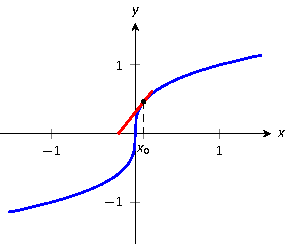
\includegraphics[scale=.75]{figures/fignewt4a}}

\subfloat[]{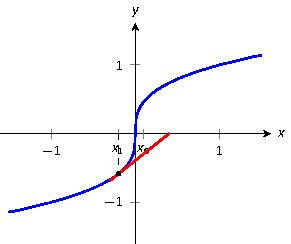
\includegraphics[scale=.75]{figures/fignewt4b}}

\subfloat[]{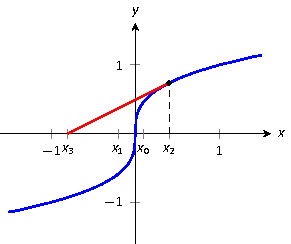
\includegraphics[scale=.75]{figures/fignewt4c}}
\caption{Newton's Method fails to find a root of $f(x) = x^{1/3}$, regardless of the choice of $x_0$.}\label{fig:newt4}
\end{center}
\end{marginfigure}

There is no ``fix'' to this problem; Newton's Method simply will not work and another method must be used.

While Newton's Method does not always work, it does work ``most of the time,'' and it is generally very fast. Once the approximations get close to the root, Newton's Method can as much as double the number of correct decimal places with each successive approximation. A course in Numerical Analysis will introduce the reader to more iterative root finding methods, as well as give greater detail about the strengths and weaknesses of Newton's Method.

%-------------
% SUMMARY
%-------------
\begin{summary} % NEED SUMMARY
\item Derivatives and tangent lines can be used to approximate the solutions of an equation.  Create successive approximations iteratively; given an approximation $x_n$, compute the next approximation $x_{n+1}$ as $$x_{n+1} = x_n - \frac{f(x_n)}{\fp(x_n)}.$$
\end{summary}

\clearpage

%--------------
% EXERCISES
%--------------
\begin{adjustwidth*}{}{-2.25in}
\textbf{{\large Exercises}}
\setlength{\columnsep}{25pt}
\begin{multicols*}{2}
\noindent Terms and Concepts \small
\begin{enumerate}[1)]
\item T/F: Given a function $f(x)$, Newton's Method produces an exact solution to $f(x) = 0$.
\item T/F: In order to get a solution to $f(x)=0$ accurate to $d$ places after the decimal, at least $d+1$ iterations of Newton's Method must be used.
\end{enumerate} 

\noindent {\normalsize Problems} \small

\noindent{\bf In exercises 3--7, the roots of $f(x)$ are known or are easily found. Use 5 iterations of Newton's Method with the given initial approximation to approximate the root. Compare it to the known value of the root.}

\begin{enumerate}[1),resume]
\item $f(x) = \cos x$, $x_0=1.5$
\item $f(x) = \sin x$, $x_0=1$
\item $f(x) = x^2+x-2$, $x_0=0$
\item $f(x) = x^2-2$, $x_0=1.5$
\item $f(x) = \ln x$, $x_0=2$
\end{enumerate}

\noindent{\bf In exercises 8--11, use Newton's Method to approximate all roots of the given functions accurate to 3 places after the decimal.
If an interval is given, find only the roots that lie in that interval.}

\begin{enumerate}[1),resume]
\item $f(x) = x^3+5x^2-x-1$
\item $f(x) = x^4+2x^3-7x^2-x+5$
\item $f(x) = x^{17}-2x^{13}-10x^8+10$ on $(-2,2)$
\item $f(x) = x^2\cos x + (x-1)\sin x$ on $(-3,3)$
\end{enumerate}

\noindent{\bf In exercises 12--15, use Newton's Method to approximate when the given functions are equal, accurate to 3 places after the decimal.}

\begin{enumerate}[1),resume]
\item $f(x) = x^2$, $g(x) = \cos x$
\item $f(x) = x^2-1$, $g(x) = \sin x$
\item $f(x) = e^{x^2}$, $g(x) = \cos x$
\item $f(x) = x$, $g(x) = \tan x$ on $[-6,6]$

\item Why does Newton's Method fail in finding a root of $f(x) = x^3-3x^2+x+3$ when $x_0=1$?

\item Why does Newton's Method fail in finding a root of $f(x) = -17x^4+130x^3-301x^2+156x+156$ when $x_0=1$?

\item A rectangular piece of cardboard of dimensions $8\times 17$
is used to make an open-top box by cutting out a small square of side
$x$ from each corner and bending up the sides. 
If $x=2$, then the volume of the box is $2\cdot 4\cdot 13=104$. Use
Newton's method to find a value of $x$ for which the box has volume
100, accurate to 3 significant figures.
%\begin{answer} $2.19$ or $1.26$
%\end{answer}

\end{enumerate}

%------------------------------------------
% END OF EXERCISES ON FIRST PAGE
%------------------------------------------
\end{multicols*}
\end{adjustwidth*}

\afterexercises 

\cleardoublepage